\subsection{Steganaliza statystyczna}

Proces ukrywania informacji w nośnikach cyfrowych zmienia ich właściwości statystyczne. Nośniki takie jak 
obrazy, dźwięki czy wideo mają przewidywalne wzorce, które są zakłócane przez steganografię. Dzięki temu 
stosując odpowiednie metody analizy statystycznej, można wykryć obecność ukrytych danych.


Najpopularniejszym nośnikiem steganograficznym wymienianym w literaturze są obrazy cyfrowe. Poniżej wymieniono 
najczęściej stosowane techniki steganalizy statystycznej w kontekście obrazów cyfrowych.
\begin{itemize}
    \item \textbf{Test chi-kwadrat}: Porównuje rozkład obserwowany z oczekiwanym, szczególnie skuteczny w analizie LSB replacement.
    \item \textbf{RS steganaliza}: Klasyfikuje grupy pikseli jako „regularne” lub „osobliwe” na podstawie zmian szumu po modyfikacji LSB.
    \item \textbf{Raw Quick Pair (RQP)}: Analizuje pary kolorów w obrazach 24-bitowych, które różnią się w bitach LSB.
    \item \textbf{Analiza histogramu}: Wykrywa zmiany w rozkładzie wartości pikseli lub współczynników DCT.
\end{itemize}

Metody te przy odpowiedniej adaptacji mogą być z powodzeniem stosowane do różnych typów nośników, przy odpowiedniej adaptacji.


Steganaliza statystyczna jest jedną z najczęściej wykorzystywanych metod w wykrywaniu ukrytych informacji 
w nośnikach cyfrowych. Jej popularność wynika z prostoty oraz szerokich możliwości zastosowania. Jedną 
z głównych zalet tej techniki jest jej dostępność i łatwa implementacja – narzędzia takie jak test 
chi-kwadrat czy analiza histogramu są intuicyjne w użyciu i bazują na podstawowych zasadach statystyki. 
Obciążona jest jednak różnymi ograniczeniami.

Metody steganografii są coraz to ulepszane.Na przykład adaptacyjne metody steganografii mogą działać 
w sposób nieregularny, dostosowując się do lokalnych cech nośnika, zmniejszając skuteczność narzędzi 
statystycznych. Dodatkowo, w sytuacjach, gdy gęstość ukrytych danych jest bardzo niska (np. poniżej 0,005 
bitu na piksel), techniki statystyczne często zawodzą -- zmiany są zbyt subtelne, by mogły zostać 
wykryte. Co więcej, niektóre techniki, takie jak Raw Quick Pair (RQP), mają 
ograniczone zastosowanie, np. wyłącznie w 24-bitowych obrazach kolorowych, co obniża ich wszechstronność. 
Dla nośników skompresowanych, takich jak JPEG, analiza statystyczna może być mniej skuteczna, ponieważ 
naturalne zmiany wprowadzane przez kompresję mogą maskować obecność ukrytych informacji.

Mimo to techniki steganalizy statystycznej są ciągle wykorzystywane. W praktyce często są łączone z bardziej 
zaawansowanymu metodami, takimi jak algorytmy uczenia maszynowego. 

\subsection{Analiza histogramów}
Steganaliza oparta na histogramach jest statystyczną metodą wykrywania ukrytych wiadomości w obrazach, 
które zostały zmodyfikowane za pomocą technik takich jak steganografia w najmniej znaczących bitach (LSB). 
Poniżej znajduje się opis implementacji metody z artykułu A Novel Steganalysis Method Based
on Histogram Analysis \cite{}.

\subsubsection{Algorytm}
Metoda opiera się na porównaniu histogramów obrazu wyjściowego (cover image) oraz podejrzanego obrazu 
(suspicious image). Specyficzny wzór różnic histogramów pomaga wykrywać obrazy stego (obrazy zawierające 
ukryte dane). Metodę zaprojektowano tak, aby była uniwersalna, czyli niezależna od zastosowanego algorytmu 
steganograficznego.

Algorytm polega na porównaniu histogramów obrazu bazowego ("cover") i podejrzanego ("suspicious"). 
Analiza różnic między tymi histogramami pozwala wykryć charakterystyczne wzorce wskazujące na użycie 
steganografii LSB.

Algorytm składa się z następujących kroków.
\begin{enumerate}
    \item Odczytanie podejrzanego i wyjściowego obrazu oraz zapisanie ich wartości intensywności pikseli.
    \item Obliczenie histogramów obu obrazów.
    \item Analiza różnic histogramów: Szukanie wartości sąsiednich, które mają tę samą wielkość, ale różne 
    znaki.
    \item Zliczenie takich par i porównanie wyniku z ustalonym progiem.
    \item Na podstawie wyniku określenie, czy obraz podejrzany to obraz stego, czy normalny obraz.
\end{enumerate}

\begin{figure}[h!]
    \centering
    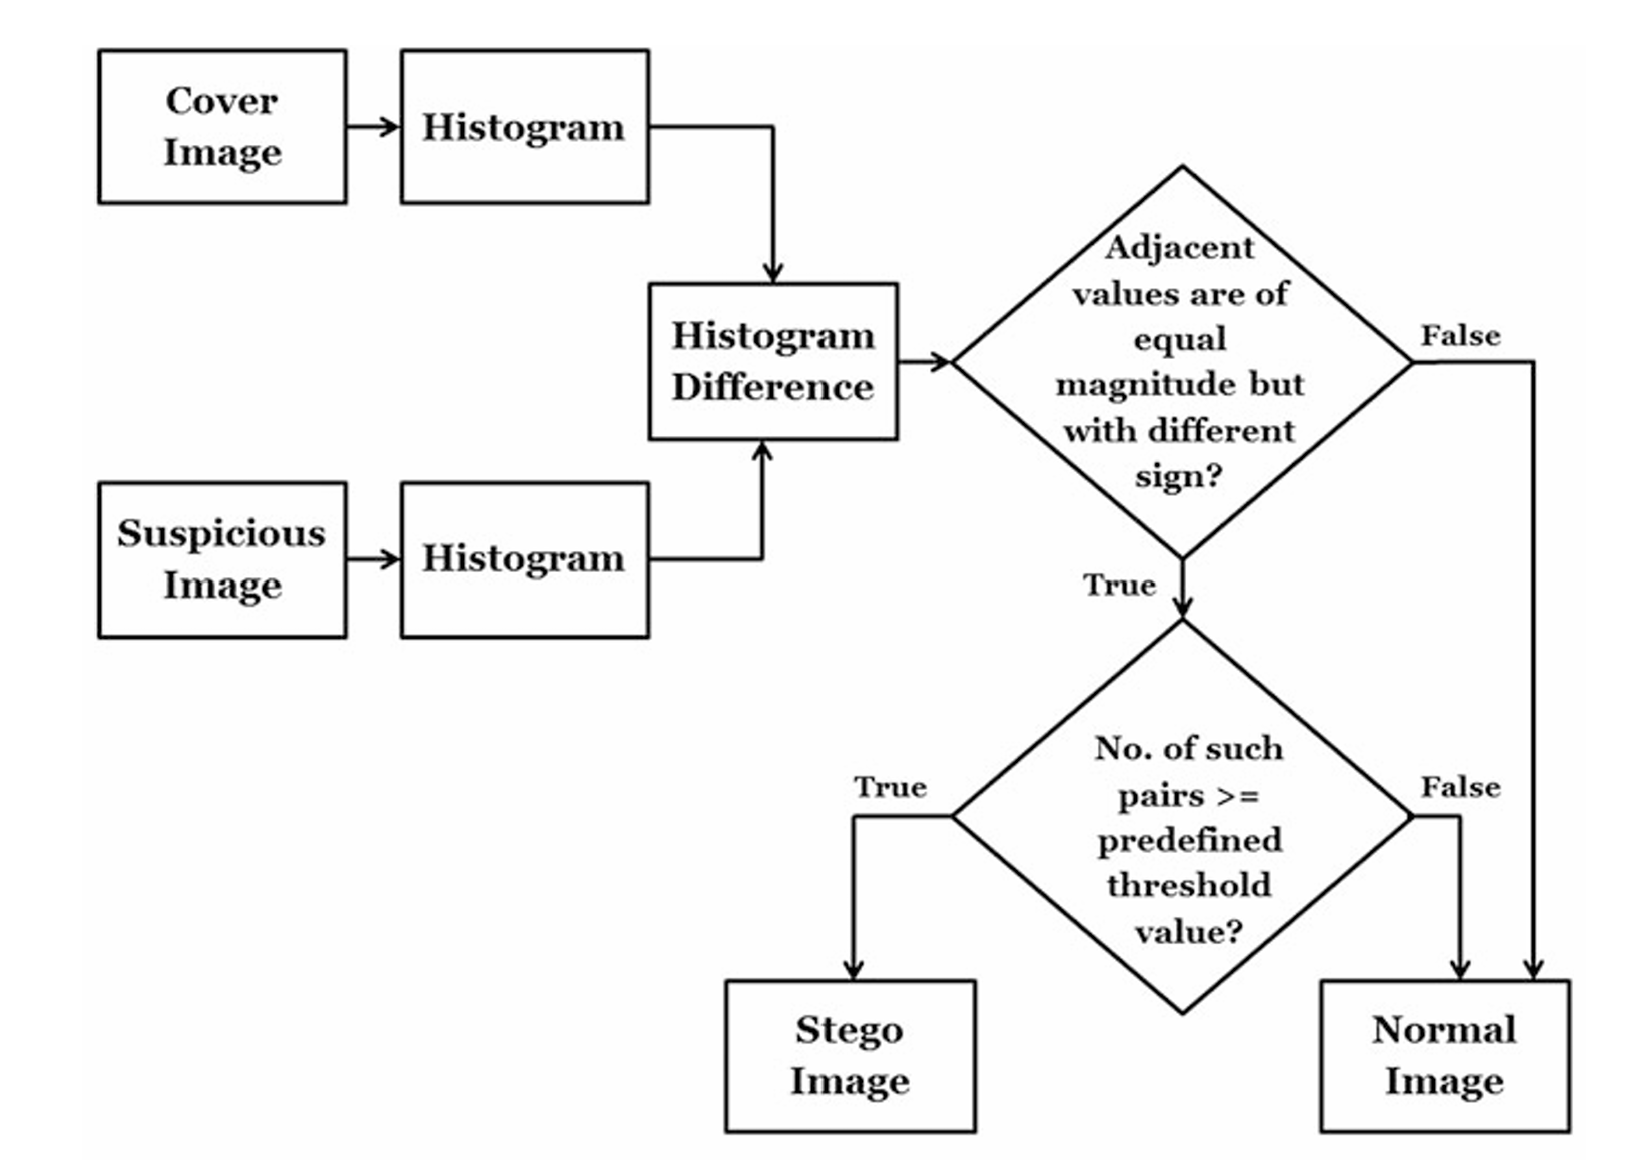
\includegraphics[width=0.8\textwidth]{./img/hist_algorythm.png}
    \caption{Schemat działania algorytmu opartego na histogramach.}
    \label{fig:histogram_algorithm}
\end{figure}
    

\subsubsection{Implementacja}
Poniżej przedstawiono fragment programu z kodem zaimplementowanego algorytmu. Pełny kod dostępny jest w 
repozytorium.

\begin{lstlisting}[language=Python, caption=Steganaliza oparta na histogramach w Pythonie]
import numpy as np
import matplotlib.pyplot as plt
from PIL import Image

def detect_stego_image(cover_image, suspicious_image, threshold):
    # Step 1: Wczytaj obrazy i zamień je na wartości intensywności (grayscale)
    cover = np.array(Image.open(cover_image).convert('L')) / 255.0
    suspicious = np.array(Image.open(suspicious_image).convert('L')) / 255.0

    # Step 2: Oblicz histogramy obu obrazów
    cover_histogram, _ = np.histogram(cover.flatten(), bins=256, range=(0, 1))
    suspicious_histogram, _ = np.histogram(suspicious.flatten(), bins=256, range=(0, 1))

    # Step 3: Wykres histogramów i różnice
    plt.bar(range(256), cover_histogram, alpha=0.5, label='Cover Image Histogram')
    plt.bar(range(256), suspicious_histogram, alpha=0.5, label='Suspicious Image Histogram')
    plt.legend()
    plt.title("Histogram Comparison")
    plt.xlabel("Pixel Intensity")
    plt.ylabel("Frequency")
    #plt.show()

    # Step 4: Różnice histogramów
    differences = suspicious_histogram - cover_histogram

    # Step 5: Zlicz różnice z przeciwnym znakiem i tą samą wartością (z tolerancją)
    counter = 0
    tolerance = 1e-6  # Tolerancja dla numerycznych błędów
    for i in range(len(differences) - 1):
        if abs(differences[i] + differences[i + 1]) < tolerance and abs(differences[i]) > 0:
            counter += 1

    # Step 6: Sprawdzenie wartości progowej licznika
    if counter > threshold:
        return True  # Stego Image
    else:
        return False  # Normal Image
\end{lstlisting}

Analizę wykonano dla próbek 20 obrazów stego i 20 obrazów cover pobranych z bazy BOSSBase. W celu sprawdzenia 
wrażliwości algorytmu na modyfikacje obrazów nie będące działaniami steganograficznymi, pliki cover poddano 
kompresji oraz wprowadzono losowy szum--w ten sposób otrzymano 20 próbek "compress".

Program sprawdził pary obrazów cover--stego oraz cover--compres i zwrócił wynik detekcji dla różnych 
wartości progu detekcji.

\subsubsection{Wyniki}

Obrazy histogramów dla jednej z 20 par przedstawiono poniżej.
\begin{figure}[h!]
    \centering
    \includegraphics[width=0.8\textwidth]{./img/compress_histogram.png_histogram.png}
    \caption{Porównanie histogramów obrazu cover i compress.}
    \label{fig:histogram_comparison}
\end{figure}
   
\begin{figure}[h!]
    \centering
    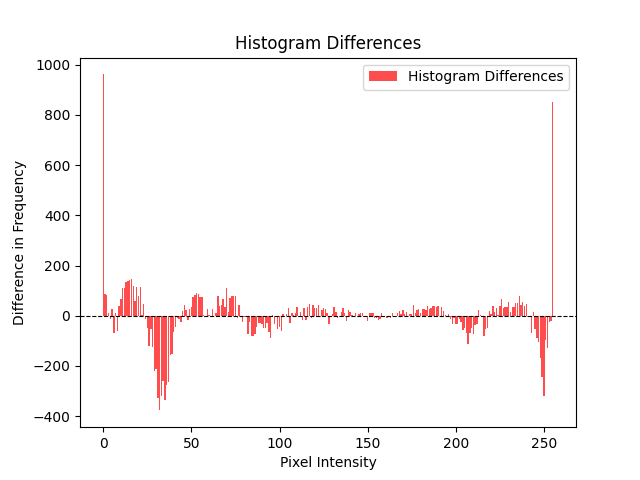
\includegraphics[width=0.8\textwidth]{./img/compress_diff_histogram.png}
    \caption{Histogram różnic między obrazami cover i compress.}
    \label{fig:histogram_diff}

\end{figure}\begin{figure}[h!]
    \centering
    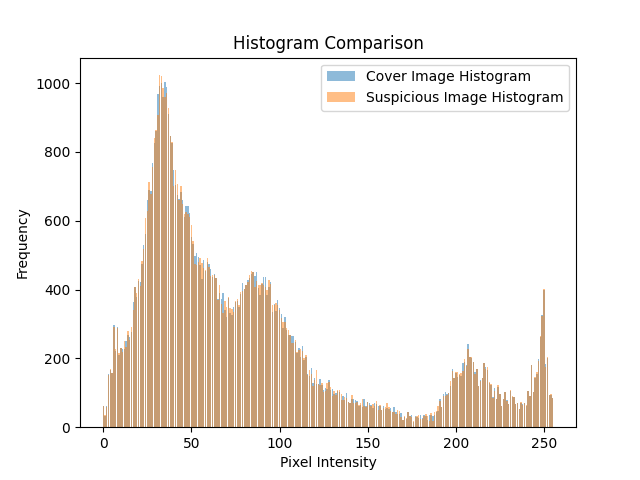
\includegraphics[width=0.8\textwidth]{./img/cover_histogram.png}
    \caption{Porównanie histogramów obrazu cover i suspicious.}
    \label{fig:histogram_comparison}
\end{figure}
   
\begin{figure}[h!]
    \centering
    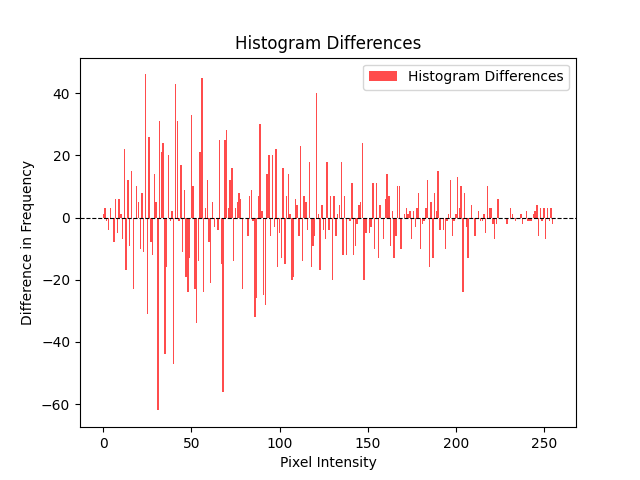
\includegraphics[width=0.8\textwidth]{./img/diff_histogram.png}
    \caption{Histogram różnic między obrazami cover i suspicious.}
    \label{fig:histogram_diff}
\end{figure}

\begin{table}[h!]
    \centering
    \begin{tabular}{@{}lccc@{}}
    \toprule
    \textbf{Próg detekcji} & \textbf{Poprawnie zidentyfikowane\\obrazy compress} & \textbf{Poprawnie zidentyfikowane\\obrazy stego} \\ \midrule
    5 & 19 / 20 & 18 / 20 \\
    6 & 19 / 20 & 16 / 20 \\
    4 & 18 / 20 & 19 / 20 \\ \bottomrule
    \end{tabular}
    \caption{wyniki klasyfikacji dla różnych progów detekcji.}
    \label{tab:classification_results}
    \end{table}

\subsubsection{Dyskusja i wnioski} 
Wyniki wyglądają bardzo dobrze. Program poprawnie zidentyfikował większość próbel. Sam algorytm był łatwy w 
implementacji oraz intuicyjny. Jest równiez prosty i nie wymaga zaawansowanych obliczeń, dlatego analiza trwa 
krótko.
Dobrze też wypada wrażliwość na szum--mimo wprowadzenia zmian do obrazów, które nie były ukrytymi 
wiadomościami, algorytm poprawnie zidentyfikował je jako obrazyy nie-stego.

Nie znany jest rodzaj steganografii, który został zastosowany do obrazów, więc nie można jednoznacznie określić 
uniwersalności metody. 

Minusem algorytmu jest to, że opiera się na porównaniu podejrzanego obrazu z oryginałem. W praktyce utrudnieniem 
może być konieczność posiadania obrazu wzorcowego. Skutecznośc zależy od ustawienia wartości progowej, co 
również może być problematyczne.

\subsubsection{Podsumowanie}
ALgorytm zaproponowany przez autorów artykułu okazał się skuteczny w wykrywaniu obrazów stego. Istnieje też 
szansa rozwoju go na analizę steganografii nie tylko przestrzennej, ale też czasowej, co pozwoliłoby na rozszerzenie 
analiz na inne nośniki cyfrowe, takie jak dźwięk czy wideo.

